\chapter{Potentials of 0$\degree$ Contact Angle Droplets}
\hspace{0em}\indent My supervisor envisions that the local properties of droplets can be revealed within a charge distribution model, which has a geometric scaling similarity to distant droplets. This chapter follows his framework, develops electric potentials for several cases, applies conformal mapping techniques and establishes the non-obvious complex potential of the conducting thin film.

Additionally, it should be noted that the derived functions in this chapter are inconsistent with similar models in \citet{Griffiths_2017} and have been incorporated into more complex scenarios.


\section{Problem Formulation}
\subsection{The Electrode, Dielectric, and Droplet Problem}
\hspace{0em}\indent Consider a droplet situated on a dielectric layer, with electrodes charging the droplet/layer and altering the droplet curve's shape and contact angle, as shown in Figure \ref{fig:sketch electrode}.
    \begin{figure}[H]
        \centering
                \adjustbox{frame=.01pt,frame,margin=.01, color=mycolor}{
        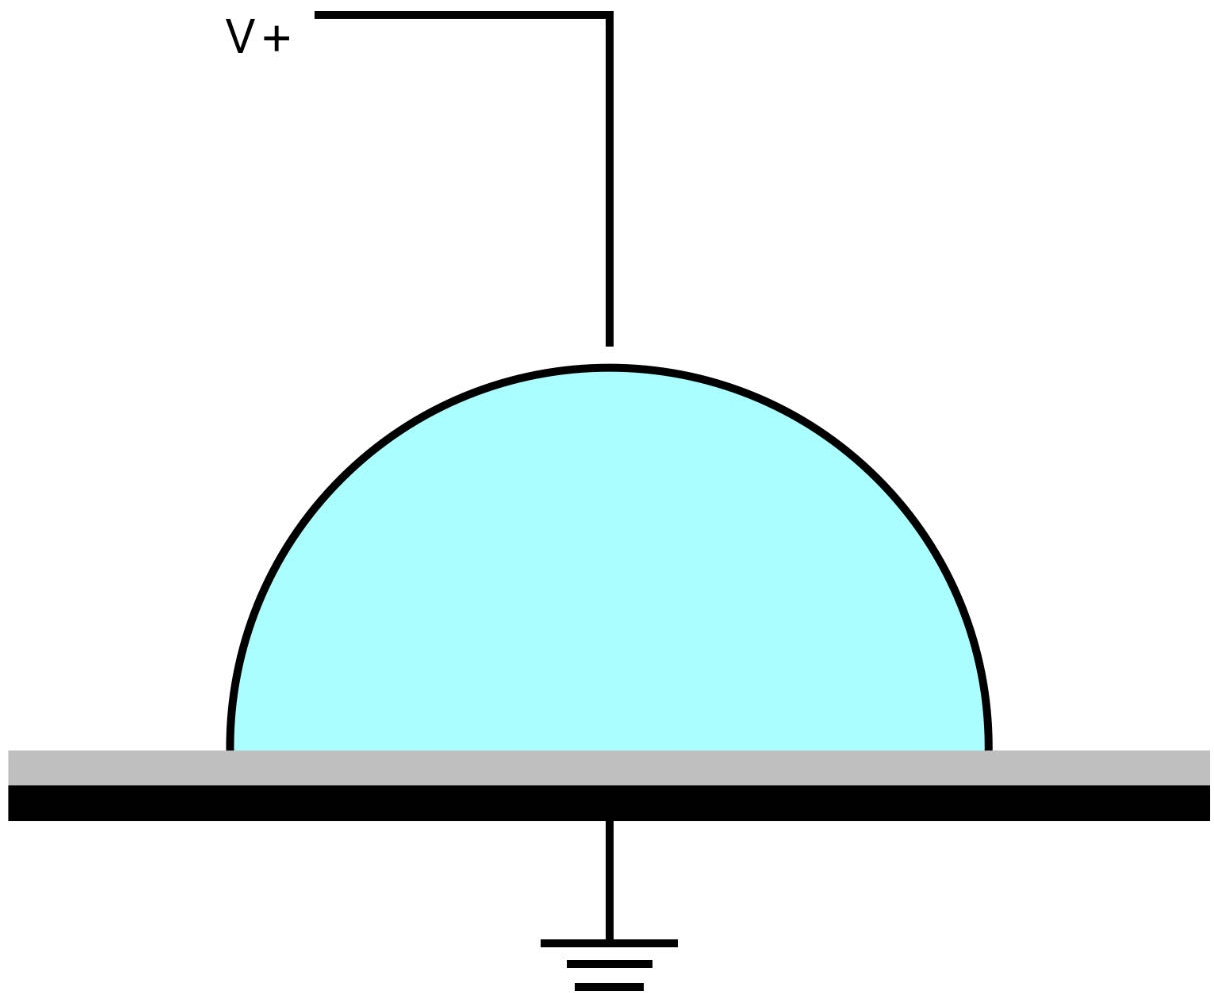
\includegraphics[width=0.7\linewidth]{Figs/sketch eletrode}}
        \caption{\small Sketch of the electrode, dielectric, and droplet problem. The $V_+$ electrode and grounded substrate create a voltage difference across the conducting droplet and layer.}
        \label{fig:sketch electrode}
    \end{figure}
Given the complexity of the functionalisation of the droplet's surface and other related issues, directly obtaining an analytical solution for its electric potential is difficult.

\subsection{The Simplification of the Problem}
\hspace{0em}\indent This study simplifies the problem in several stages. First, when observed from a distance, the droplet's shape degenerates into a thin film with negligible height, which we refer to as a ``slit". The dielectric layer is assumed to be semi-infinite in $-y$ and $\pm x$ directions relative to the slit. Second, the influence of the electrodes is simplified to a point charge, though its precise location and magnitude are not accurately depicted in the following figure, as these parameters may vary. Figure \ref{fig:slit} provides an approximate representation of the simplified Situation.

Additional characteristics of the simplified configuration include the surface charge on the boundary of the dielectric layer, the volume charge within the dielectric, and the voltage at infinity. The latter remains unknown and, at this stage, cannot be constrained in a manner that satisfies the uniqueness theorem (section \ref{thm:uniquenss}).

    \begin{figure}[H]
        \centering
        \adjustbox{frame=0.25pt,frame,margin=0.15,color=mycolor}{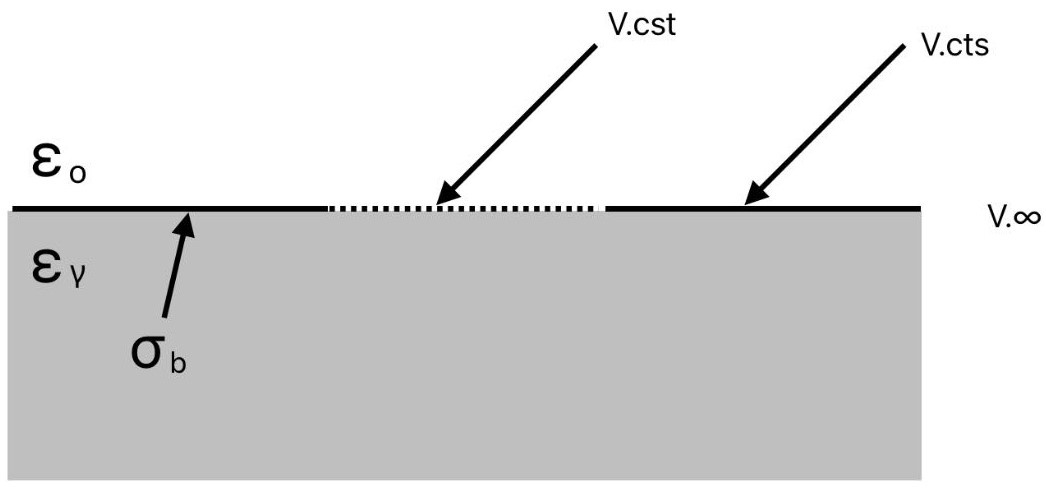
\includegraphics[width=.8\linewidth]{Figs/slit_e.jpg}}
        \caption{\small Thin droplet slit on the dielectric layer. The dashed line represents the slit, while the thick black lines indicate the boundaries of the dielectric and the air above. The shaded areas denote the dielectric, and the upper space of air is left blank. Additionally, $\epsilon_0$ and $\epsilon_{\gamma}$ are the electric permittivity of air and the dielectric, respectively. $\sigma_b$ is the surface charge density of the dielectric layer, with the surface charge density in the air is set to be zero. V.cst indicates the slit is itself an equipotential surface, V.cts means the voltage is continuous along the dielectric-air interface, and V.$\infty$ represents the far-field voltage, which is unknown.\\
        Lastly, it should be noted that we use a point charge to represent the electrodes, which is not shown in the sketch. This point charge is embedded somewhere in the dielectric and varies in magnitude due to the properties of the electrodes.}
        \label{fig:slit}
    \end{figure}
For other properties and coefficients not explicitly included in the sketch, we can now establish the boundary conditions:
\begin{itemize}
    \item All charges of the conductive droplet $\Omega$ are distributed along the boundary of the droplet.
    \vspace{-0.5em}
   \[\int_{\partial \mathcal{D}} \sigma_{\partial\Omega} \df l = Q_{\Omega}\vspace{-0.5em}
   \]
    \item There is an induced volume charge density $\rho$ at $\vec{r_0}$ in the dielectric, where the embedded point charge is located.
    \[
    \epsilon_0\nabla\cdot \mathbf{E}=\frac{q}{\epsilon_r}\delta(\vec{r}-\vec{r}_0)%\vspace{-1em}
    \]
    \item Except for the location of the embedded point charge, all induced charges in the dielectric $\mathcal{D}$ are distributed along the boundary of the dielectric and the air.
    \vspace{-.5em}
     \[\nabla\cdot \mathbf{E}=0\hspace{1em}\text{s.t. in }\mathcal{D}\setminus \{\partial \mathcal{D} \cup \vec{r}_0\}\vspace{-1em}\]
    \item The voltage of the conducting droplet is constant.
    \vspace{-0.5em}
    \[V(\Omega)=Constant\vspace{-1em}\]
    \item The voltage is continuous on the boundary $\partial \Omega$. The voltage $V^{(b)}$ represents that in the dielectric, and the air above has a voltage $V^{(a)}$ .
    \begin{equation}\label{eqn:v.cts}
\left.V^{(a)}\right|_{\partial\mathcal{D}^+}=\left.V^{(b)}\right|_{\partial\mathcal{D}^-}        
    \end{equation}
\end{itemize}
\vspace{-.5em}
\hspace{0em}\indent Yet some uncertain properties at this stage include:
\begin{itemize}
    \item There may be induced charges at the boundary $\partial\mathcal{D}$, caused by the presence of free charge(the point charge). let $\l^o$ be a small closed loop across the boundary $\partial\mathcal{D}$; Gauss's Law states that 
    \[\oint_{l^o} -\epsilon \nabla V\cdot\hat{n}\df l = \pi r^2\sigma_b\]
    or in terms of $\vec{E}$, since the boundary lies along the $x$-axis, only the $y$ component of $\vec{E}$ contributes:
    \begin{equation}\label{eqn:gauss}
    \epsilon_0 E^{(a)}_y-\epsilon_\gamma E^{(b)}_y=\sigma_b   
    \end{equation}
    
    However, charge distributions with no induced charge on the boundary between the dielectric and the space above do exist, as a later case shows.
    
    \item We are generally uncertain about the exact behaviour at infinity.  Besides the far-field voltage of a point charge, the voltage at infinity does not necessarily decrease, the semi-infinite dielectric may contribute.

    \item The equipotentials around the slit are unknown, as are those around the two cusps. Additionally, the induced charge of the slit mixes with that of the dielectric at the slit's lower boundary line\(\partial\Omega \cap \partial\mathcal{D}\).
\end{itemize}

although the droplet's height is ignored, the electric potential of the simplified problem remains challenging due to the boundary conditions.

\subsection{Apply the Joukowski Transformation}\label{cpt:jkw}

\hspace{0em}\indent The Joukowski transformation maps the slit to a disc. If we can determine an appropriate electric potential for the embedded disc, dielectric, and point charge scenario, we can use the inverse map to address the cusps. However, this approach introduces a new challenge due to the asymmetric dielectric geometry relative to the y-axis, as outlined in Figure \ref{fig: maped disc}.

\begin{figure}[H]
    \centering
    \adjustbox{frame=0.25pt,frame,margin=0.15,color=mycolor}{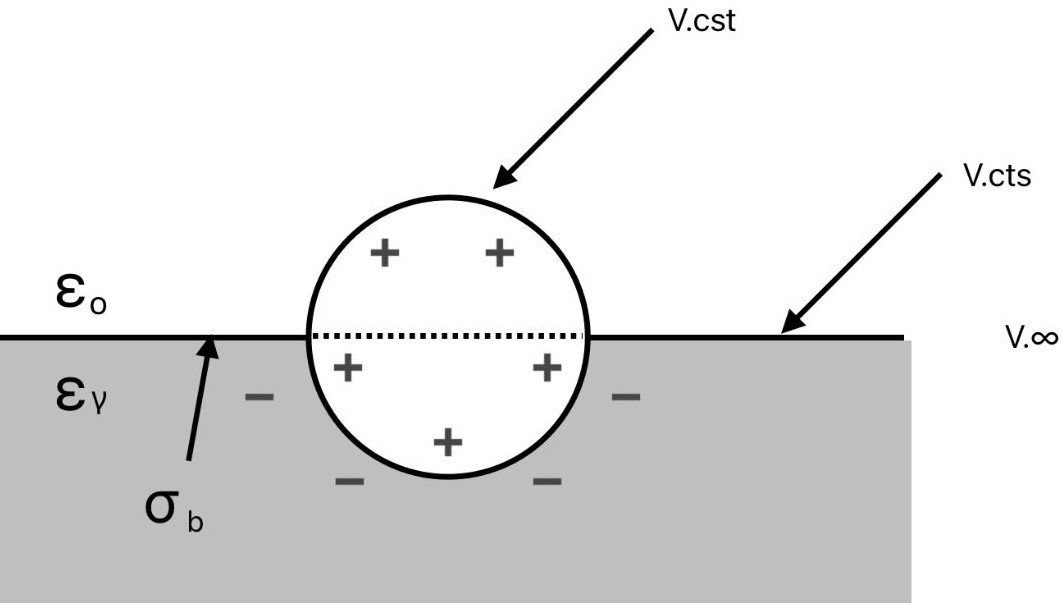
\includegraphics[width=.8\linewidth]{Figs/disk.jpg}}
    \caption{\small The problem corresponds to the Joukowski transformation. In addition to the previously included parameters, the $+$ and $-$ signs represent the surface charge distributions on the disc and the dielectric boundary in contact with it.}
    \label{fig: maped disc}
\end{figure}
the corresponding boundary conditions include:
\begin{itemize}

    \item $\nabla^2 w = 0$ except at boundary lines and the location of the point charge, where $w$ is the complex potential.
    
    \item At $|\zeta|\leq1$, $\Im [w]=0$. This represents the $V(\Omega)$ condition.
    
    \item at $\zeta\in\mathbb{R}$, $\Im [w_a]=\Im [w_b]$, representing the continuous voltage condition on the boundary in the complex plane.
    
\end{itemize}
Hence, we are eventually facing a Laplace equation/Poisson equation problem.

\section{Analyzing the Component Electrical Models}
\subsection{Charged Disc Embedded in Dielectric: A Point Charge-like Electric Field}\label{cpt:charged disc}
\hspace{0em}\indent Consider a disc of radius $R=1$, charged with $q$, embedded in a semi-infinite dielectric. let $\theta_s$ be the arc of the disc in contact with the dielectric.

The dielectric structure is symmetric about $\theta_s$, which corresponds to the right angle at the contact point in Figure \ref{fig:disk in D}. However, it allows for variation in how much the disc is embedded, as measured by the parameter $\theta_s$.
\begin{figure}[H]
    \centering
    \adjustbox{frame=0.25pt,frame,margin=0.15pt,color=mycolor}{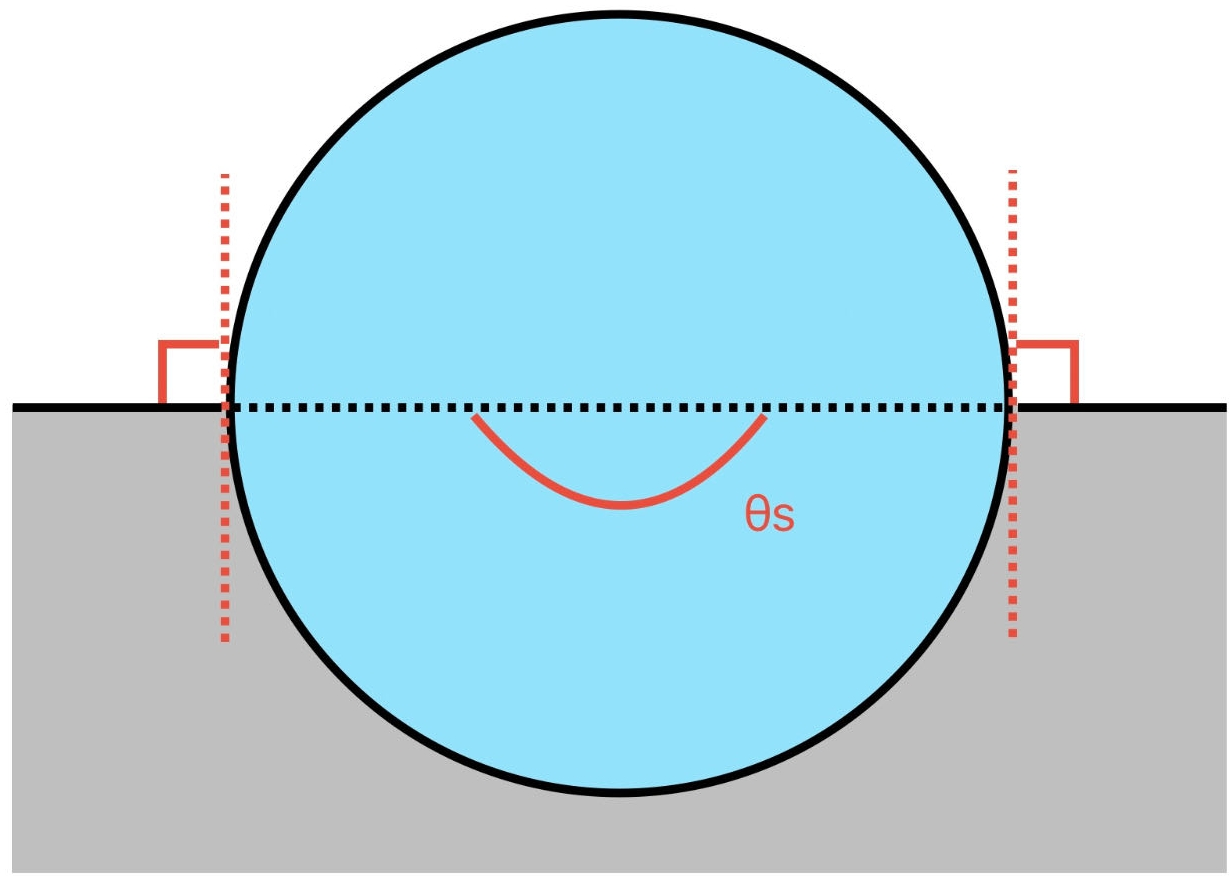
\includegraphics[width=0.46\linewidth]{Figs/sketch disk embedded right.jpg}}\hfill
    \adjustbox{frame=0.25pt,frame,margin=0.15pt,color=mycolor}{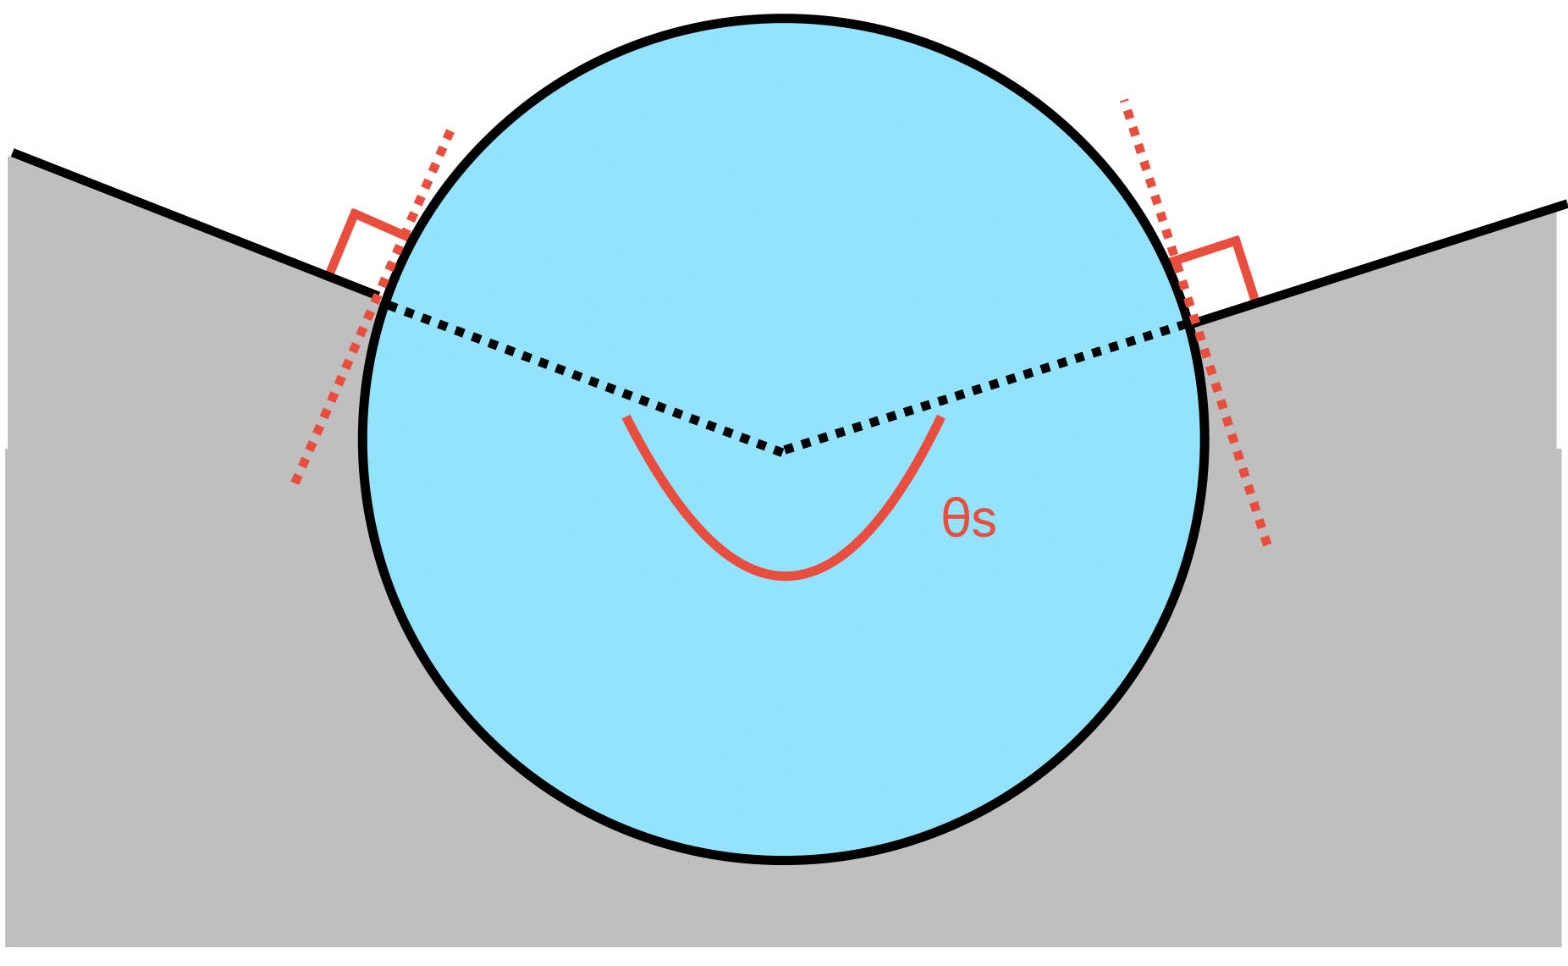
\includegraphics[width=0.531\linewidth]{Figs/sketch disk embedded angle.jpg}} % Side by side images
    
    \caption{\small Two cases are presented where the disc is embedded in a dielectric, measured by $\theta_s$. The left figure shows the case where $\theta_s=\pi$, while the right figure depicts a different $\theta_s$. It is found that the electric fields of the cases differ based on $\theta_s$.}
    \label{fig:disk in D}
\end{figure}

Postulate that the far-field voltage is 
\[V_{\infty}=  \frac{q'}{2\pi\epsilon_0} \log r\]
where $q'\not\equiv q$ is some magnitude of charge. If the voltage satisfies the necessary local boundary conditions, we can be confident that this is the correct voltage for the configuration according to the uniqueness theorem (\ref{uniqueness}).

On the boundary between the droplet and the dielectric, $R=1, \theta\in(0\footnote{Let the point where the dielectric contacts the disc from the left be the zero angle.}, \theta_s)$. According to equation (\ref{eqn:die surf q}),
\[
\sigma_b = \vec{P}\cdot\hat{n}=\epsilon_0 \chi_e E_{\hat{r}}
\]
where\footnote{Note that along the arc, the normal direction of the dielectric boundary points toward the origin. Let the disc be positively charged; the electric field of the disc points outward. Also, note that the sum of the induced surface charge (from both the dielectric and the disc) is positive, with its own electric field lines pointing outward, which is why there are two minus signs in equation (\ref{eqn:surf dq}). }
\begin{equation}\label{eqn:surf dq}
    E_{\hat{r}} = -E_{q} - \frac{\sigma_b}{2 \epsilon_0}  
\end{equation}
Hence
\[
\sigma_b= \epsilon_0 \chi_e \left( -\frac{q}{2 \pi R \epsilon_0} - \frac{\sigma_b}{2 \epsilon_0} \right)
\Longrightarrow \sigma_b = -\frac{q}{2 \pi R} \cdot \frac{2 \chi_e}{2 + \chi_e}
\]
Postulate that the surface charge density in the dielectric\footnote{At the contact line of the dielectric and the disc, the total surface charge density is the sum of both.} on the arc at $R=1$ is uniformly $\sigma_b$, then the total surface charge $q_s$ is
\[\sigma_b \int^{\theta_s} R\df\theta= -q \frac{2 \chi_e}{2 + \chi_e}\cdot\frac{\theta_s}{2 \pi} =q_s\]
let $\theta_s=\pi$ in our case, the total charge $q_t$ of the system is then
\begin{equation}\label{eqn:disk,d,qt}
    q_t=q+q_s=q(1-\frac{1}{2}\frac{2\chi_e}{2+\chi_e})=q\frac{2}{2+\chi_e}\leq q
\end{equation}
The electric field is unique everywhere, regardless of whether it is in the dielectric or not:
\[
\vec{E}=\frac{q_t}{2\pi\epsilon_0 r}\hat{r}=\frac{q}{2\pi\epsilon_0 r}\frac{2}{2+\chi_e}\hat{r}
\]
and the voltage is:
\[
v=\frac{1}{2\pi\epsilon_0}\frac{2q}{2+\chi_e}\log r
\]
The electric field is symmetric about the origin; its field lines parallel to the dielectric boundary along $\pm x$. Hence, the dielectric contains no surface charge other than $\sigma_b$ on the arc.

The surface charge distribution on the disc, $\sigma_d$, is then
\begin{align*}
\sigma_d&= \begin{cases}q_t/\pi &, \theta\in(0,\pi) \\
|\sigma_b| + q_t/\pi &,  \theta\in(\pi,2\pi)\end{cases}
\end{align*}

\subsection{Point Charge Embedded in Dielectric: Different Electric Fields in Various Regions}\label{cpt:charge in die}
\hspace{0em}\indent For a point charge embedded in a dielectric below the $x$-axis, the three types of charges in this setup are the free charge, the induced volume charge, and the induced surface charge.

The free charge $q_f$ is simply the point charge $q$. The point charge induces a volume charge density $\rho_b$ at $\vec{r}_0(x,y) = (0, -d)$, \[q_b=\int_\mathcal{V}\rho_b\Longleftrightarrow \rho_b = q_b\delta(\vec{r}-\vec{r}_0)
\]
and an induced surface charge density $\sigma_b$.

The two quantities need to be determined to satisfy the following boundary conditions, equation (\ref{eqn:v.cts}), which ensures continuity in voltage, and equation (\ref{eqn:gauss}), which applies Gauss's Law to the surface charge density.

The electric field consists of two different components. For the voltage inside the dielectric, we treat the charge and the induced volume charge field as a single entity $q$, Gauss's Law provides:
\[
V = \frac{q}{2\pi\epsilon} \log(r - r_0)
\]
where $\epsilon$ is the permittivity.

By method of Image, we replace the dielectric with induced charges and treat all charges as if they were in a vacuum, using $\epsilon_0$, hence 
\[V_{q}=\frac{q}{2\pi\epsilon_0} \log(r-r_0)\]
and
\[V_{q_b}=\frac{q_b}{2\pi\epsilon_0} \log(r-r_0)\]
By equation (\ref{eqn:P}), $\vec{P}=\epsilon\chi_e \vec{E}$, and equation (\ref{eqn:rho_b}), $\rho_b\coloneqq-\nabla\cdot\vec{P}$,
\[q_b\coloneqq\int_{\mathcal{V}} \rho_b\delta (\vec{r}-\vec{r}_0)=-\frac{\chi_e}{1+\chi_e}q\Longrightarrow q+q_b=\frac{1}{1+\chi_e}q=\frac{q}{\epsilon_r}
\]
the two voltages sum to
\[
V=V_q+V_{q_b}=\frac{1}{2\pi\epsilon_0}\frac{q}{\epsilon_r}\log (r-r_0)=\frac{1}{2\pi\epsilon_0}\frac{q}{\epsilon_r}\log\sqrt{(x-0)^2+(y--d)^2}
\]
the electric field pointing $\hat{y}$ is
\[
E_y=-\frac{\partial V}{\partial y}=\frac{1}{2\pi\epsilon}\frac{q}{\sqrt{(x)^2+(y+d)^2}}\frac{1}{\sqrt{(x)^2+(y+d)^2}}\frac{1}{2}2(y+d)=\frac{1}{2\pi\epsilon}\frac{q(y+d)}{x^2+(y+d)^2}
\]
at $y=0$
\[
E_q=\frac{1}{2\pi\epsilon}\frac{qd}{x^2+d^2}=\frac{1}{2\pi\epsilon_0}\frac{1}{1+\chi_e}\frac{qd}{x^2+d^2}
\]
by equation (\ref{eqn:ed.line}), surface charge density satisfies
\[
E_\sigma=-\frac{\sigma_b}{2\epsilon_0}
\]
and by equation (\ref{eqn:rho_b}), $\sigma_b=\vec{P}\cdot\hat{n}=\epsilon_0\chi_e\vec{E}\cdot\hat{n}$, from the two we find
    \[    \sigma_b=\epsilon_0\chi_e\left(E_q+E_{\sigma}\right)=\epsilon_0\chi_e\left(\frac{1}{2\pi\epsilon_0}\frac{1}{1+\chi_e}\frac{qd}{x^2+d^2}-\frac{\sigma_b}{2\epsilon_0}\right)\Longrightarrow
        \frac{2+\chi_e}{2}\sigma_b=\frac{1}{2\pi}\frac{\chi_e}{1+\chi_e}\frac{qd}{x^2+d^2}
    \]
hence the induced surface charge density of the dielectric, on $y=0$, is
\[
\sigma_b=q\frac{\chi_e}{1+\chi_e}\frac{1}{2+\chi_e}\frac{ d / \pi}{x^2+d^2}
\]
\subsection{Dielectric Shielding and the Difference from \citeauthor{Griffiths_2017}}\label{cpt:shield}
\hspace{0em}\indent After deriving the electric properties for the models above, we find that our results are inconsistent with similar cases in Chapter 4 of \citet{Griffiths_2017}. In Example 4.5 on page 187, the textbook derives the case of a metal sphere charged $Q$, surrounded by dielectric of finite radius and finds that in the region $\vec{r}>\vec{r}_{\mathcal{D}}$,
\[E_{textbook}\sim Q/\epsilon_0\] 
However, using our derivation method, the electric field is found to be
\[E= \frac{1}{4 \pi r^2}\frac{Q}{\epsilon_0}\frac{2}{2+\chi_e}\] 
which is smaller by a factor $\frac{2}{2+\chi_e}$ compared to the textbook result. The other two similar cases from \citet{Griffiths_2017} are Problem 4.35, concerning a point charge in a spherical dielectric; and Problem 4.38, regarding a conducting sphere embedded in a dielectric\footnote{See \citet{Griffiths_2017}, Ex. 4.5, p. 187 and Problem 4.35, p. 206, for reference.}.

In these cases, the textbook derives without considering certain surface charge densities. All our results are smaller by a factor of $\frac{2}{2+\chi_e}$, and the details of calculations are omitted here.

Hence we need to examine carefully if they match the required local boundary conditions in our situation. For the point charge in the dielectric case, we check whether the integral of the surface charge density, $q_s$, cancels out the induced volume charge $q_b$
\[
q_s\coloneqq\int_S \sigma_b \df a \Longrightarrow \int_\mathbb{R}\sigma_b \df x=q\frac{1}{1+\chi_e}\frac{\chi_e}{2+\chi_e}\frac{d}{\pi}\int_\mathbb{R}\frac{1}{x^2+d^2}\df x=...\frac{d}{\pi} \frac{\pi}{d}=q\frac{\chi_e}{1+\chi_e}\frac{1}{2+\chi_e}
\]
Yet the amount of induced volume charge is:
\begin{equation}\label{eqn:sigma_b}
q_b=\int_\mathcal{V}-\nabla\cdot\vec{P}=-\nabla\cdot\epsilon_0\frac{\chi_e}{\epsilon}\vec{D}=- q\frac{\chi_e}{1+\chi_e}    
\end{equation}
we observe that $q_s \neq q_b$. If they were equal, it would almost imply that, when observed from the outside, the dielectric appears to have no effect\footnote{Which is the scenario presented in \citet{Griffiths_2017} examples, and is not in this thesis. The derivation follows.}. Since this is not the case, we must locate the surplus charge to determine the dielectric's actual effect in the situation. 

The voltage below is the potential due to three point charges. The charges $q_f$ and $q_b$ at $(x,y) = (0,-d)$, sum to
\[
q_r=q_f + q_b = (1-\frac{\chi_e}{1+\chi_e} )q =\frac{1}{1+\chi_e}q=\frac{q}{\epsilon_r}
\]
and the induced surface charge sums to $q_s$. We locate it at $(x,y)=(0,d)$. The voltage below the $x$-axis is therefore
\begin{align*}
    V_{below}&=\frac{1}{2\pi\epsilon_0}\left(q_r\log\sqrt{x^2+(y+d)^2} +q_s\log\sqrt{x^2+(y-d)^2}\right)
    \\&=\frac{q}{2\pi\epsilon_0}\left(\frac{1}{\epsilon_r}\log\sqrt{x^2+(y+d)^2} +\frac{\epsilon_r-1}{\epsilon_r}\frac{1}{\epsilon_r+1}\log\sqrt{x^2+(y-d)^2}\right)
    \\&=\frac{q}{2\pi\epsilon_0}\left(\frac{1}{\chi_e +1}\log\sqrt{x^2+(y+d)^2} +\frac{\chi_e}{1+\chi_e}\frac{1}{2+\chi_e}\log\sqrt{x^2+(y-d)^2}\right)    
    \\&=\frac{q}{2\pi\epsilon_0\epsilon_r}\left(\log\sqrt{x^2+(y+d)^2} +\frac{\chi_e}{2+\chi_e}\log\sqrt{x^2+(y-d)^2}\right)    
    \end{align*}

For the voltage above the $x$-axis, locate $q_s$ at $(x,y) = (0,-d)$, while the other two remain at their original positions. The three charges sum to
\[q_t=
q_o+q_b+q_s=\frac{q}{\epsilon_r}+\frac{q}{\epsilon_r}\frac{\chi_e}{2+\chi_e}=\frac{q}{1+\chi_e}\frac{2+2\chi_e}{2+\chi_e}=\frac{2q}{\chi_e+2}
\]
hence the voltage is
\[
V_{above}=\frac{1}{2\pi\epsilon_0}\frac{2 q}{({\chi_e+2})}\log\sqrt{x^2+(y+d)^2}=\frac{q}{\pi\epsilon_0}\frac{1}{(\epsilon_r+1)}\log\sqrt{x^2+(y+d)^2}
\]
Moreover, check if Gauss's Law satisfies
\begin{align*}
\frac{\partial V_{above}}{\partial y}-\frac{\partial V_{below}}{\partial y}&=\frac{q}{2\pi} \left( \frac{2}{\epsilon_r + 1} \frac{y + d}{x^2 + (y + d)^2} - \frac{1}{\epsilon_r} \frac{y + d}{x^2 + (y + d)^2} -\frac{1}{\epsilon_r} \frac{\epsilon_r-1}{\epsilon_r+1}\frac{y - d}{x^2 + (y - d)^2}\right)   
\end{align*}
at $y=0$
\begin{align*}
\left.\frac{\partial V_{upper}}{\partial y}-\frac{\partial V_{lower}}{\partial y}\right|_{y=0}&=\frac{q}{2\pi} \frac{d}{x^2 + d^2}\left( \frac{2}{\epsilon_r + 1} - \frac{1}{\epsilon_r} +\frac{1}{\epsilon_r}\frac{\epsilon_r-1}{\epsilon_r + 1}  \right) \\
    &=\frac{q}{2\pi}  \frac{d}{x^2 + d^2}  \frac{2\epsilon_r -\epsilon_r -1+\epsilon_r -1}{\epsilon_r(\epsilon_r + 1)} \\
    &=\frac{q}{2\pi}  \frac{d}{x^2 + d^2} \frac{2\epsilon_r -2}{\epsilon_r(\epsilon_r + 1)} \\
    &=\frac{q}{\pi}  \frac{d}{x^2 + d^2} \frac{\epsilon_r -1}{\epsilon_r(\epsilon_r + 1)}=\frac{q}{\pi}  \frac{d}{x^2 + d^2}\frac{\chi_e}{\chi_e +1}\frac{1}{\chi_e +2}
\end{align*}

It matches $\sigma_b$ in equation \ref{eqn:sigma_b}; Gauss's Law is fulfilled\footnote{For further confirmation, see a related problem at \citet{Griffiths_2017} Ex 4.25, p. 207.}. 

The voltage $V_{above}$ describes how the dielectric affects the surroundings. We observe that the apparent magnitude of the charge $q_s$ varies, yet it retains the form of a point charge with a fixed location. Consequently, the problem of the point charge, dielectric, and droplet reduces to that of a point charge field, differing only in the charge magnitude, which is advantageous.

Furthermore, an interesting phenomenon was observed: the voltage outside the dielectric is not as commonly expected, as though the dielectric had no effect at all:
\[
V_{expected}=\frac{q}{2\pi\epsilon_0}\log\sqrt{x^2+(y+d)^2}
\]
implies the dielectric leaves no effect on the external  region\footnote{If this were true, we receive two electric signals from the same charge, once sent from the vacuum, and once enclosed by dielectric before sending. There will be no difference between the two.}.  

Our derivation shows the quantity of a charge embedded in a dielectric, as seen from outside, is less than it actually is.
\[
\frac{V_{upper}}{V_{expected}}=\frac{q}{\pi\epsilon_0(\epsilon_r+1)} / \frac{q}{2\pi\epsilon_0}=\frac{2}{1+\chi_e+1}\leq 1\vspace{3em}
\]
Physically, this claims the dielectric shields some of the electric energy of embedded charges, which sounds plausible. The equipotentials of the point charge embedded in the dielectric are as follows.
\begin{figure}[H]
    \centering
    \adjustbox{frame=0.25pt,frame,margin=0.15,color=mycolor}{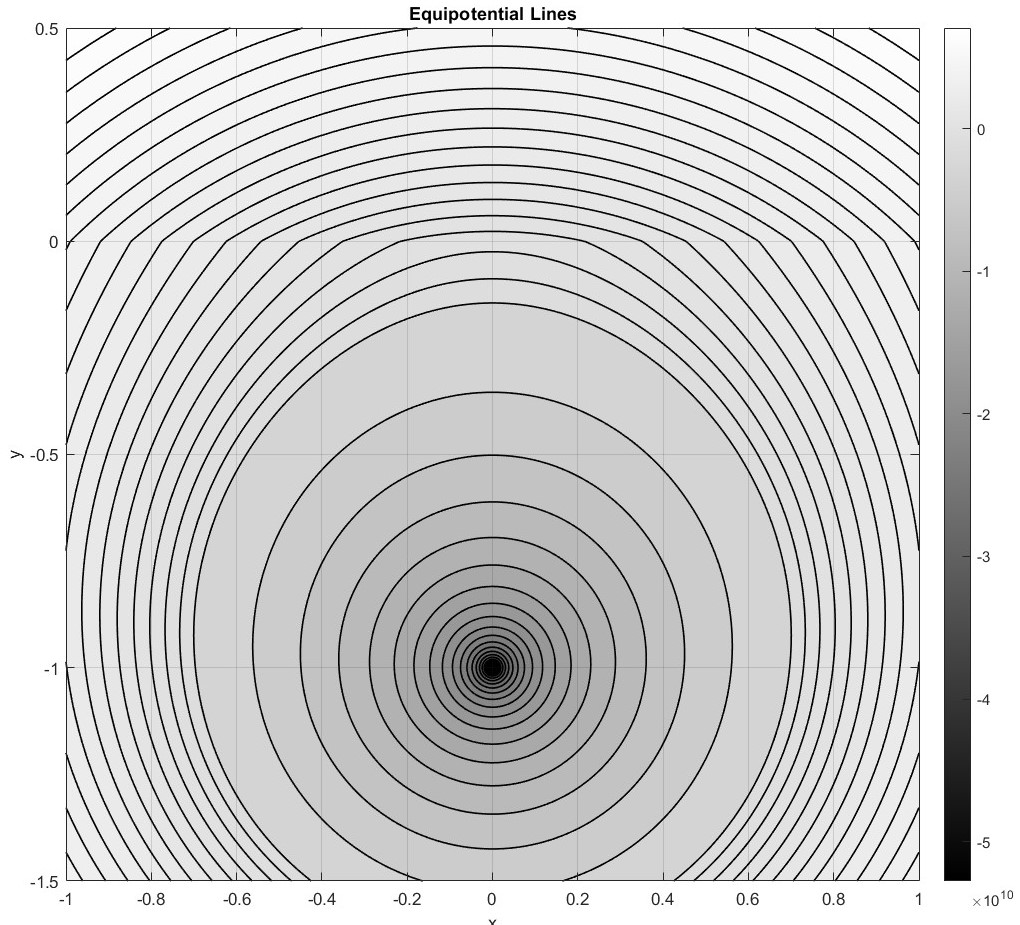
\includegraphics[width=1.\linewidth]{Figs/dieletic potential.jpg}}
    \caption{\small The equipotentials of a point charge embedded in the dielectric exhibit a noticeable change in direction at \(y=0\), which is the boundary between the dielectric and the air above. This indicates that the electric field is disrupted while the potential remains continuous due to the induced surface charge. In the region \(y>0\), the potential forms concentric circular equipotential lines created by a charge located at \(y=-d\), which has a smaller magnitude than the actual charge.
 }
    \label{fig:enter-label}
\end{figure}

In the case of a charged disc embedded in a dielectric, we find that $q_t\leq q$ in equation (\ref{eqn:disk,d,qt}), which also demonstrates the shielding effect.
\section{The Potential of the Charge, Dielectric, and Disc Problem}
\subsection{The Complex Potential of the Disc}
\hspace{0em}\indent For a typical complex potential, it is free to use either the real or imaginary part to be the voltage. However, we will set the imaginary part as the voltage, because we require $r=1$ to be an equipotential, $\Im \left[w(|\zeta|=1)\right]=0$ , by adding $\overline{w}(\zeta^{-1})$. The complex potential of the charge is\vspace{-1.em}
\[
w_0(\zeta)=\im \log (\zeta-\zeta_0)\vspace{-1.5em}
\]
and adding
\[
\overline{w_0}(\frac{1}{\zeta}) = -\im \log (\frac{1}{\zeta}-\Bar{\zeta_0})
\]
This generates two physical entities: a sink $-\im\log (1-\zeta\zeta_0)$ at $1/\overline{\zeta_0}$ , and a source $\im\log(\zeta)$ at $\zeta = 0$ . For a point charge at \(\zeta_\alpha\) and for the unit circle to be an equipotential, two extra charges of opposite sign must be added.

\subsection{The Induced Charges of the Dielectric}
% The effect of the charges in the dielectric is investigated using conformal mapping and yields surprising results that may help understand the properties of this geometric form of a dielectric.
\hspace{0em}\indent 
The disc induces two charges inside, which may affect the dielectric and therefore require investigation. The charge at \(\zeta = 0\) does not influence the dielectric except on the arc, as proved in section (\ref{cpt:charged disc}). However, the charge at \(1/\overline{\zeta_\alpha}\) may induce surface charge in the dielectric. 

Suppose the charge in the disc off the origin induces a charge in the dielectric; it will induce two more charges inside the disc, the twice-induced charges. As this process continues, the voltage will evolve into a series\vspace{-0.5em}
\[
q\log (\zeta-\zeta_{\alpha})+\frac{q}{\epsilon}\log (\zeta-\zeta_1)+\frac{q}{\epsilon^2}\log (\zeta-\zeta_2)+...\vspace{-0.5em}
\]

The dielectric is not flat, and we are uncertain about the possibly induced charge. To determine the possible induced charge, map the surface of the dielectric to a flat one, with
\[\zeta=z-\sqrt{z^2-1}\]
\begin{figure}[H]
    \centering
    \adjustbox{frame=0.25pt,frame,margin=0.15,color=mycolor}{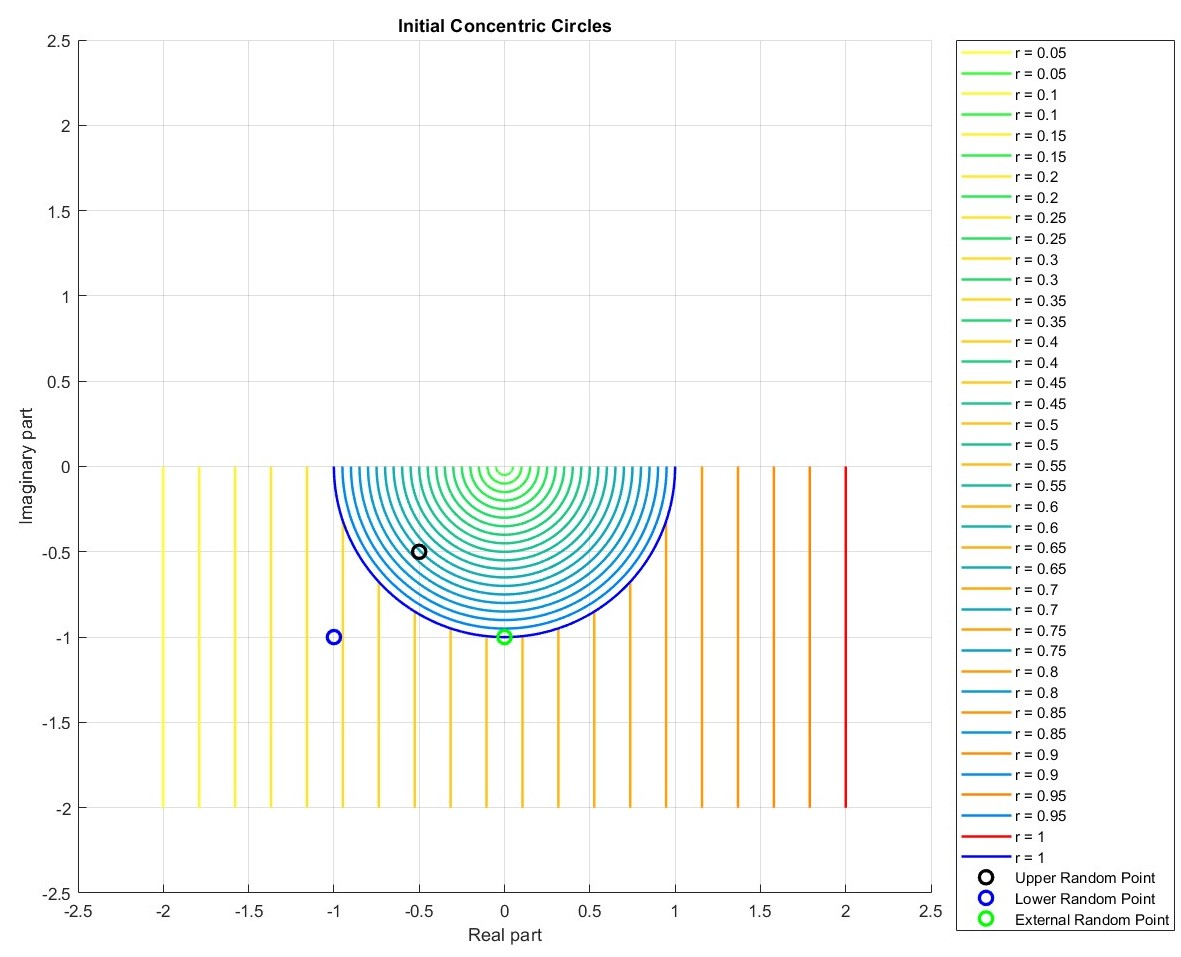
\includegraphics[width=0.493\linewidth]{Figs/semi circle and dieletric}}\hfill
    \adjustbox{frame=0.25pt,frame,margin=0.15,color=mycolor}{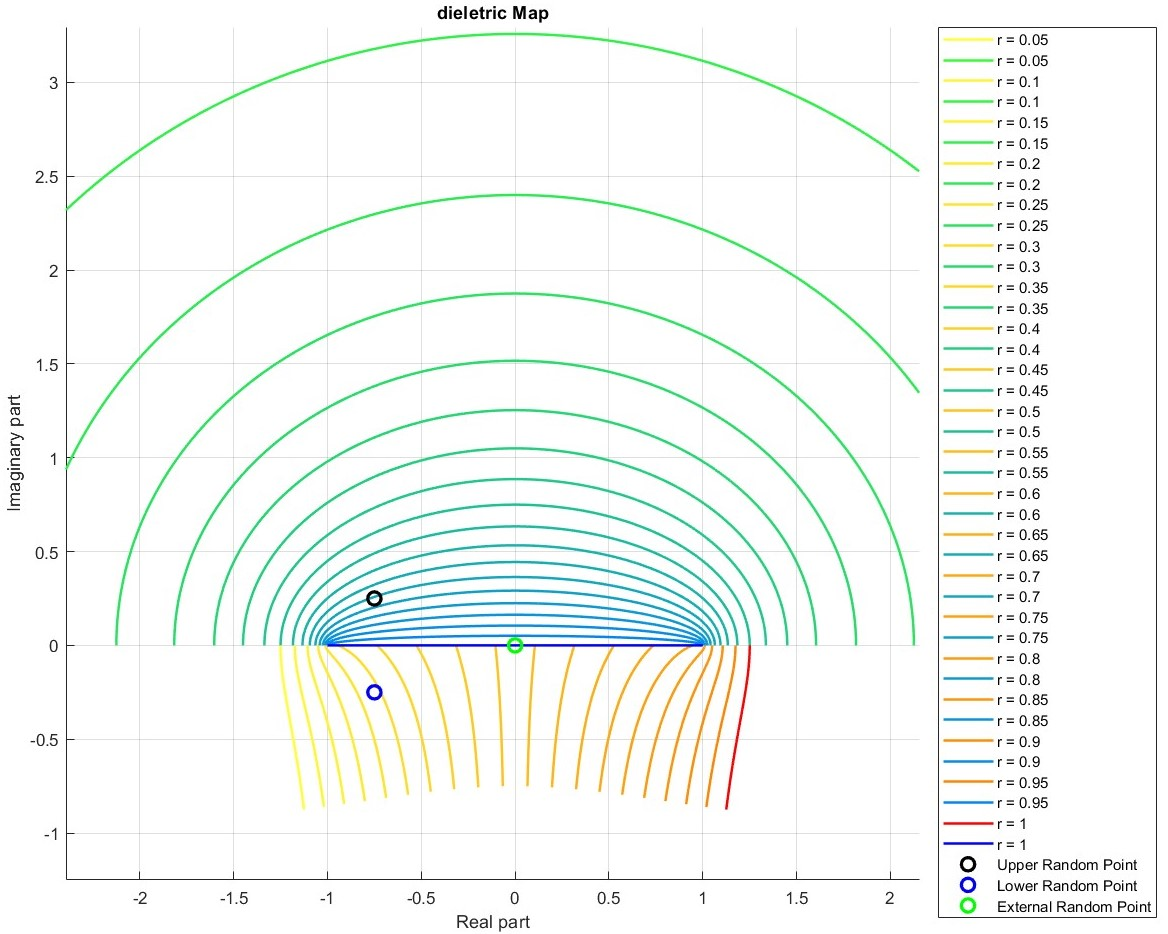
\includegraphics[width=0.5\linewidth]{Figs/map flat dieletric}} % Side by side images
    \caption{\small The point charge (the blue circle) and one of the induced charges (the black circle) in the disc. The left figure is the $\zeta$ plane, the right figure is the $z$ plane. The lower semi-circle (green and blue lines) map to the $y>0$ space, and the dielectric (yellow and red lines) map to $y<0$. The origin $\zeta=0$ maps to $\infty$, which fits the physical condition of the dielectric.\\
    Moreover, The dielectric area is compressed, and physically, $\epsilon$ may change, hence the dielectric is not linear anymore. This possible effect is ignored. 
}
    \label{fig:induce charge map}
\end{figure}

From the right figure of the $z$ plane, we see that the source charge (the blue circle) induced a charge (the black circle). For a point charge at $\zeta_{\alpha}=(-1-\im)$ in the dielectric, the corresponding induced charge inside the disc is at\vspace{-1.em}
\[\zeta_{o}=1/\zeta_{\alpha}=-\frac{1}{2}-\frac{1}{2}\im\vspace{-1.em}\]
and it maps to
\[
z_{o}=\frac{\zeta_{0}}{2}+\frac{1}{2 \zeta_{o}}=-\frac{3}{4}+\frac{1}{4}\im\]
Since the mapped dielectric is flat, take the conjugate to find $z_d=-\frac{3}{4}-\frac{1}{4}\im$, this is the location of the possibly twice-induced charge. The inverse map finds the twice-induced charge's location on the $\zeta$-plane is
\[
\zeta_d=z_d-\sqrt{z^2-1}=-1-\im
\]
This is where the source charge is located; hence, there will be no continuous charge generation.

The two induced charges in the complex equation are located within a conducting disc, where a real free charge cannot reside from a physics perspective. Therefore, they should represent an cumulative effect of the surface charges in the disc and induce no further charges.

\iffalse
This means the conformal mapping captures the physics property of the geometry of the dielectric. A further question is how the equipotential line requirement is fitted, as the dielectric area is rather ordinary. It will be discussed later.

The next question is, will the charge in the unit disc induce a charge in the dielectric? verified via conformal mapping, if it does, the location will be the location of the source charge. 


\begin{itemize}
    \item The induced charge of the source charge will not lie within the disc but will instead be projected onto the opposite side of the disc, and it generates a corresponding charge distribution within the conductive disc.
    \item The potential inside the dielectric is the superposition of the potentials generated by the source charge, its image charge, and the corresponding charge distribution within the disc.
    \item The potential outside the dielectric is equivalent to the potential generated by a smaller charge together with a conductive disc.
    \item The charges within the disc will not generate induced charges (either in the dielectric or elsewhere). There will be no free charges located inside the conductor, and this charge is a substitute for several induced surface charge distributions and therefore will not generate further induced charges.
\end{itemize}
Therefore, the internal voltage of the dielectric we proposed earlier is sufficient, with limited charge adjustment and compensation.

\fi

\subsection{The Potential on the $\zeta$-plane}\label{cpt:pot_zeta}
\hspace{0em}\indent The voltage has two parts, according to section (\ref{cpt:shield}). Assume the voltage in the air is the sum of a point charge (magnitude to be determined) and the induced charges in the disc. The complex potential of above is found to be\vspace{-1em}
\begin{equation}\label{eqn:w_up}
    w_{+}(\zeta) = \frac{q}{\pi \epsilon_0}\frac{1}{\epsilon_r+1} \im \left[ \log(\zeta - \zeta_0) - \log\left(\frac{1}{\zeta} - \overline{\zeta_0}\right) \right]\vspace{-1em}  
\end{equation}
\begin{figure}[H]
    \centering
    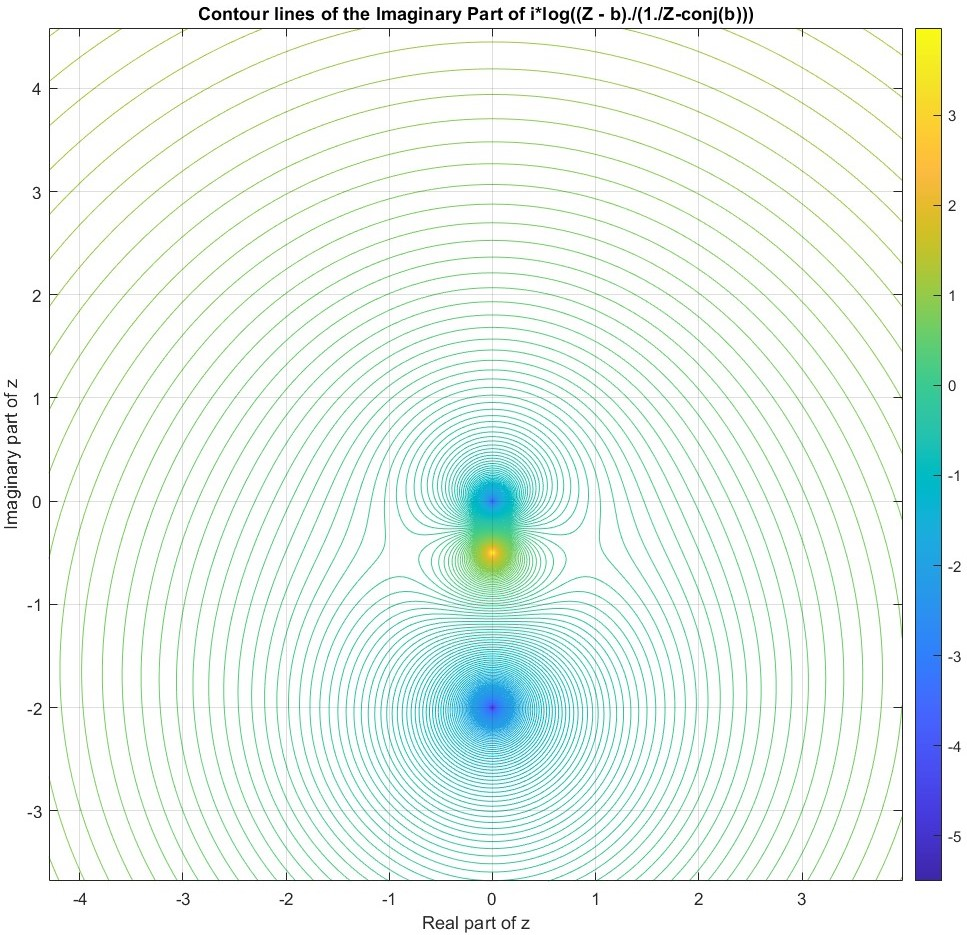
\includegraphics[width=1.\linewidth]{Figs/equal-pot, disk and charge, far view.jpg}
    \caption{\small The equipoentials from above. $y=0$ is the boundary between the dielectric and air. The three charges are the source charge at $(0, -2)$, and the two induced charge inside the disc. One at the origin, with the same sign of the source charge, and one differ. The equipoential of the disck is roughly visible.}
    \label{fig:enter-label}
\end{figure}

For the voltage below, start from charges (of different magintudes) in $W_+$, we need to determine the position and proportion the induced charge to meet the boundary conditions.

After some manipulation and trials, we derived that, the induced charge must be locate at $\overline{\zeta}_0$ above the disc. Previously, we found the structure with $q_t$ at $\overline{\zeta}_0$,  $q_b$, $q_r$ at ${\zeta}_0$ satisfies the conditions. Hence for the two charge at $\zeta_0$, and $1/\overline{\zeta_0}$, the corresponding charges must replicate the structure. Additionally, the charges at the origin do not affect surface charge distribution or the continuity of the voltage. 

\begin{figure}[H]
    \centering
    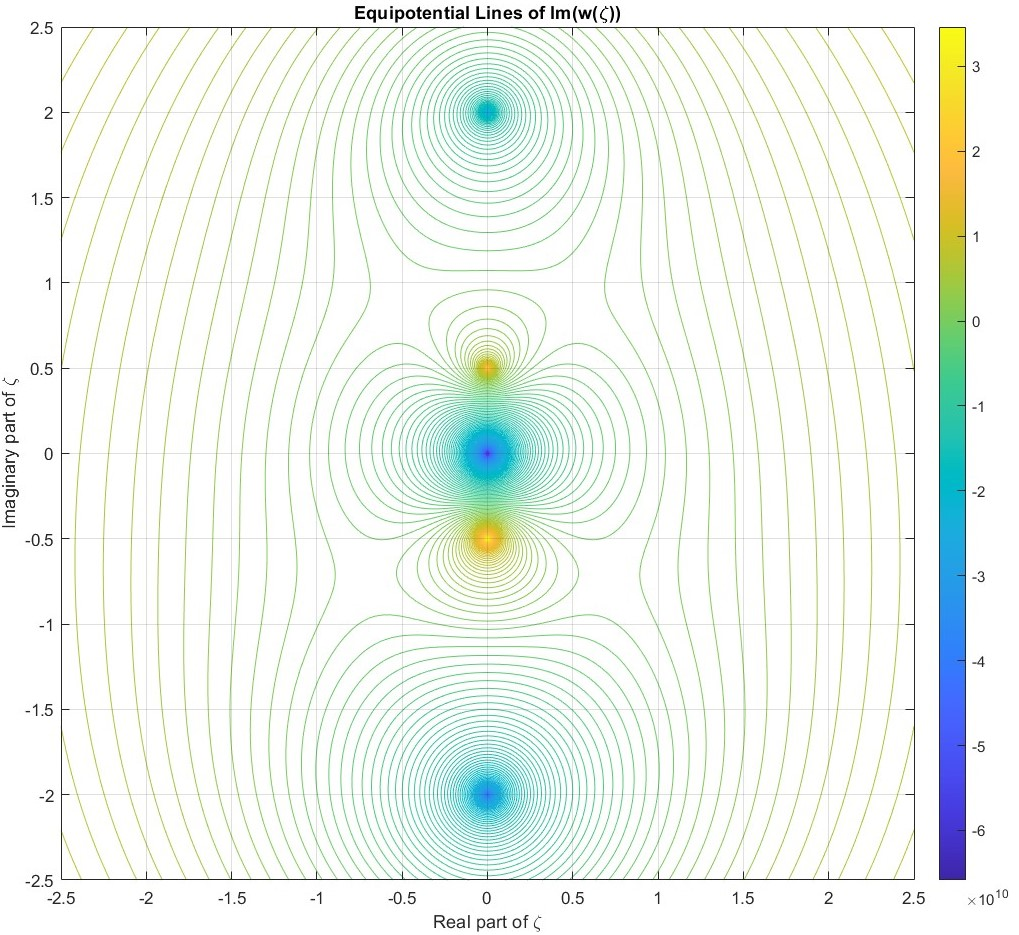
\includegraphics[width=1.\linewidth]{Figs/disc phase, inside dieletric.jpg}
    \caption{The equipotential from below. the potential contains six point charges, three of magnitude $q_b$ located separately at the source charge position, inside the semi-circle below, and the origin. Three of the fractions of the source charge $q_r$ are located symmetrically about the $y$-axis. Thus, there are two charges at the origin.}
    \label{fig:w_down}
\end{figure}


The complex potential of the dielectric area below $y=0$, of Figure (\ref{fig:w_down}) is \vspace{-.5em}
\begin{equation}\label{eqn:w_down}
    w_{-}(\zeta) = \frac{q}{2\pi \epsilon_0\epsilon_r} \im \left[ \log(\zeta - \zeta_0) - \log\left(\frac{1}{\zeta} - \overline{\zeta_0}\right) \right]
+\frac{q}{2\pi \epsilon_0\epsilon_r}\frac{\epsilon_r-1}{\epsilon_r+1}\im \left[ \log(\zeta - \overline{\zeta_0}) - \log\left(\frac{1}{\zeta} - \zeta_0\right) \right]    
\end{equation}
We check the voltage continuity at $y=0$, the other boundary conditions are satisfied simultaneously. From equation (\ref{eqn:w_up}) and equation (\ref{eqn:w_down}), \vspace{-1.em}
\[
V_+= \frac{q}{\pi \epsilon_0}\frac{1}{\epsilon_r+1} \left\{ \log\left(\sqrt{x^2+d^2}\right) -\log\left|\frac{1-\zeta\overline{\zeta_0}}{x}\right| \right\}
\]
\[
V_-= \frac{q}{2\pi \epsilon_0\epsilon_r} \left\{ \log\left(\sqrt{x^2+d^2}\right) -\log\left|\frac{1-\zeta\overline{\zeta_0}}{x}\right| \right\}
+\frac{q}{2\pi \epsilon_0\epsilon_r}\frac{\epsilon_r-1}{\epsilon_r+1} \left\{\log(\sqrt{x^2+d^2}) - \log\left|\frac{1-\zeta\zeta_0}{x}\right| \right\}
\]
We see that the three $\{...\}\coloneqq\alpha$ are equal on the $x-$axis, hence  \vspace{-1.em}
\[
V+=\frac{q}{\pi \epsilon_0}\frac{1}{\epsilon_r+1} \alpha\]
\[
V_-=\left(\frac{q}{2\pi \epsilon_0\epsilon_r} +\frac{q}{2\pi \epsilon_0\epsilon_r}\frac{\epsilon_r-1}{\epsilon_r+1}\right)\alpha
=\frac{q}{2\pi \epsilon_0\epsilon_r}\left( 1+\frac{\epsilon_r-1}{\epsilon_r+1}\right)\alpha
=\frac{q}{2\pi \epsilon_0\epsilon_r}\frac{2\epsilon_r}{\epsilon_r+1}\alpha=V_+
\]

\subsection{Mapping the Complex Potential to the $z$-plane}\label{cpt:slit_pot}
Next, we find a mapping $\zeta(z)$ from the semi-circle above to the slit, as Figure \ref{fig:map above} shows. The desired complex potential on the $z$-plane would be $w(\zeta(z))$.\vspace{-0.5em}
\begin{figure}[H]
    \centering
\adjustbox{frame=0.25pt,frame,margin=0.15,color=mycolor}{
    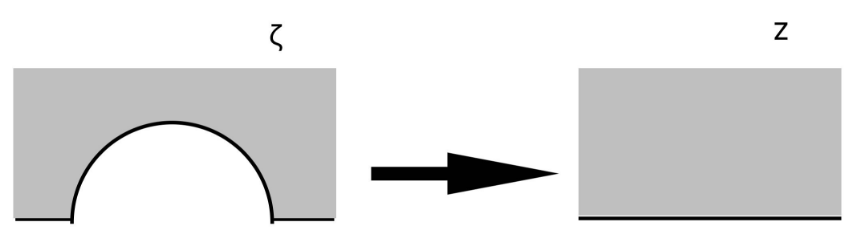
\includegraphics[width=1.\linewidth]{Figs/slit map brief.png}}
    \caption{\small The Mapping to addressing the charge, dielectric and slit problem. the shaded area represents the air and the upper arc of the disc, corresponding to the upper edge of the slit.}
    \label{fig:map above}
\end{figure}
\vspace{-0.5em}
In Matlab, $\zeta=z-\sqrt{z^2-1}
$ maps the left half of $\zeta$ plane, except the unit disc, to the left half of $z$ plane, and $\zeta=z+\sqrt{z^2-1}$ maps the right half of the $\zeta$ plane, except for the unit disc, to the right half of $z$ plane. Following the setting in Matlab, the complex potential on the $z$-plane is therefore divided into four parts.

Figure \ref{fig:vz above} is the equipotential of the voltage in the region $y>0$, on the $z$-plane\footnote{The $w(r<1)$ region must be excluded in the mapping. For an incorrect example see Appendix \ref{fig:wrong pot}.}. 

\begin{figure}[H]
    \centering
    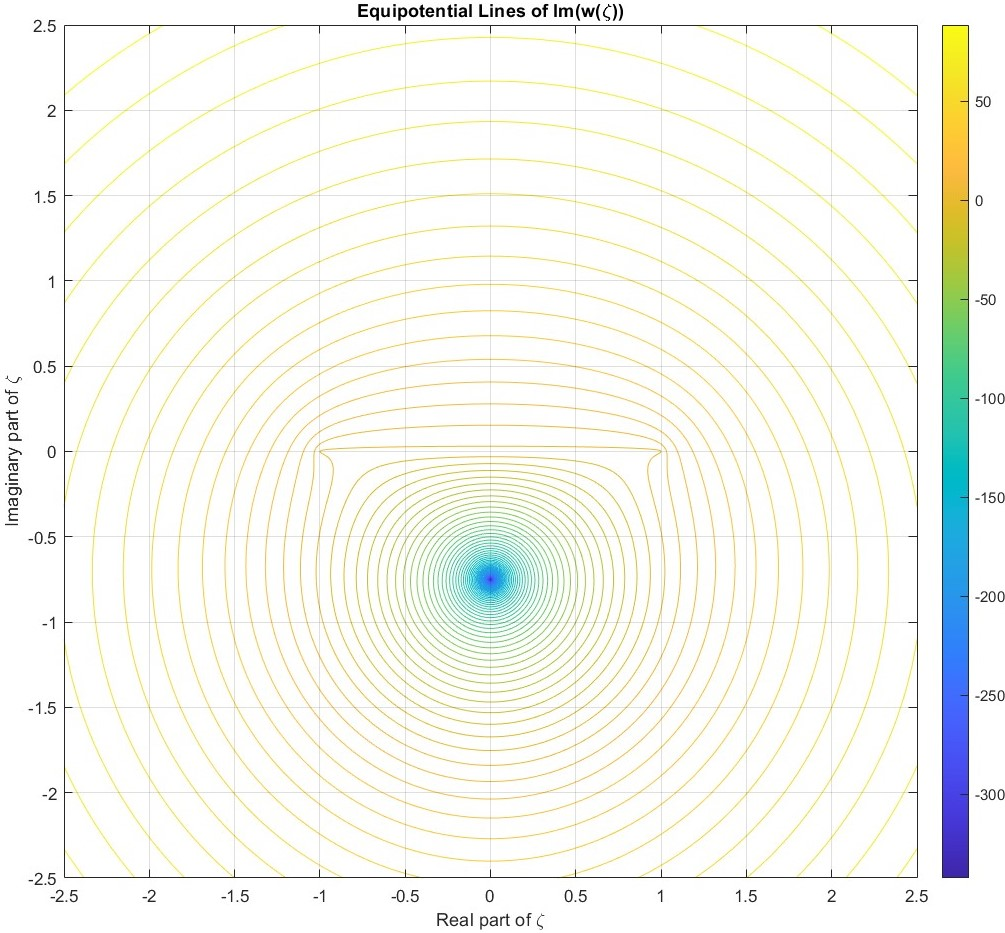
\includegraphics[width=1.\linewidth]{Figs/slit, Pot out dielectric, right.jpg}
    \caption{\small The equipotential lines of the area $y>0$, the 1, 2 quadrants. The dielectric is located in the region $y<0$. The slit is at $(x\in\pm1,y=0)$, and there is one equipotential intersect the slit. This is analogous  to streamline of a vortex under the slit of fluid dynamic. The source charge is at the centre of the concentric circles inside the dielectric.}
    \label{fig:vz above}
\end{figure}
For the complex potential above on the $z$-plane, start from equation (\ref{eqn:w_up}), leave $\zeta_0$ unchanged, use $\zeta(z)$ replacing $\zeta$ to rewrite $w(\zeta)$. In the first quadrant $(x>0, y>0)$, the complex potential is\vspace{-0.5em}
\[
\prescript{1}{}{w_{+}(z)} =\frac{q}{\pi\epsilon_0\epsilon_r}  \im \left[\log\left(z+\sqrt{z^2-1} - \zeta_0\right) - \log\left(\frac{1}{z+\sqrt{z^2-1}} - \overline{\zeta_0}\right)\right] \vspace{-0.5em}
\]
and in the second quadrant$(x<0, y>0)$, \vspace{-0.5em}
\[
\prescript{2}{}{w_{+}(z)} = \im \left[\log\left(z-\sqrt{z^2-1} - \zeta_0\right) - \log\left(\frac{1}{z-\sqrt{z^2-1}} - \overline{\zeta_0}\right)\right] \vspace{-2.em}
\]
    \begin{figure}[H]
        \centering
        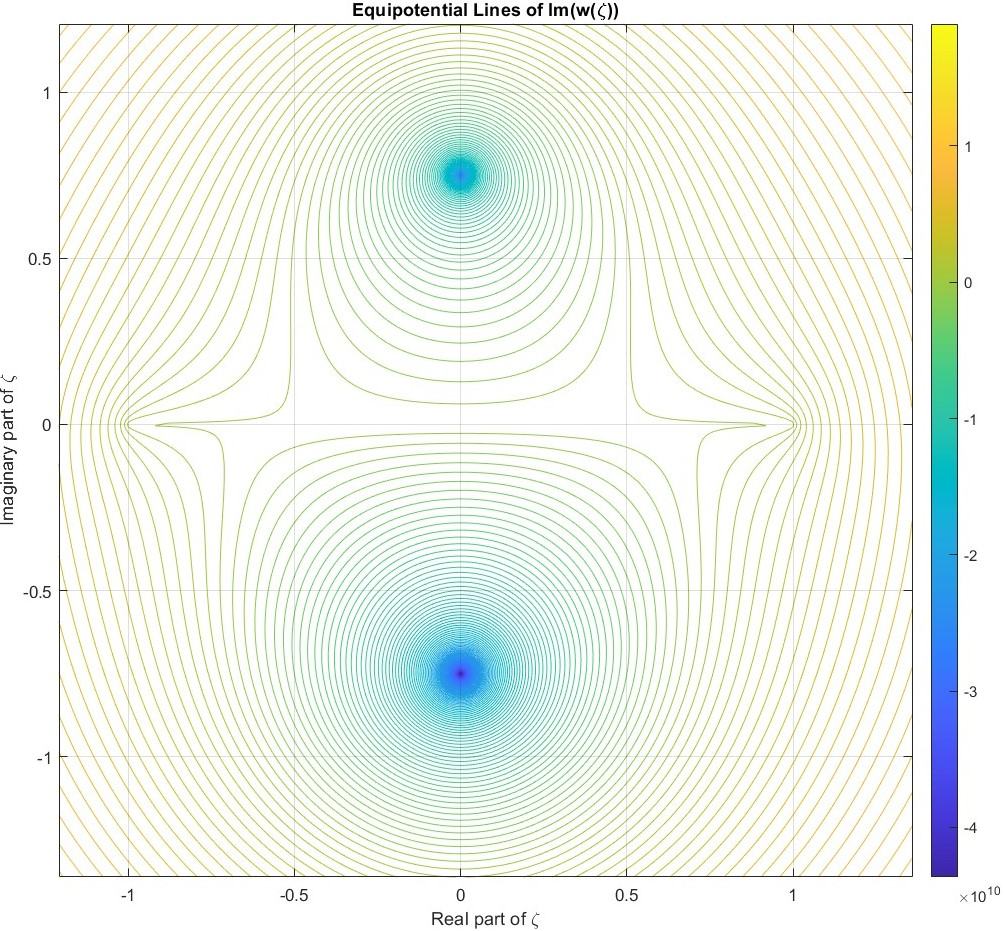
\includegraphics[width=1.\linewidth]{Figs/disc phase, inside dieletric, maped.jpg}
        \caption{\small The equipotentials in the region $y<0$, the 3, 4 quadrants. There is an induced charge above the dielectric. The slit is at $(x\in\pm1,y=0)$. One equipotential line reaches the slit, and the dense lines around the two cusps resemble the flow past a slit in fluid dynamics.}
        \label{fig:enter-label}
    \end{figure}\vspace{-1.em}
In the third quadrant$(x<0,y<0)$ and the fourth quadrant$(x>0,y<0)$, by equation (\ref{eqn:w_down}), we find the complex potentials are\vspace{-0.5em}:
\begin{align*}
\prescript{3}{}{w_{-}(z)} &= \frac{q}{2\pi \epsilon_0\epsilon_r} \im \left[ \log(z-\sqrt{z^2-1} - \zeta_0) - \log\left(\frac{1}{z-\sqrt{z^2-1}} - \overline{\zeta_0}\right) \right]\\
&+\frac{q}{2\pi \epsilon_0\epsilon_r}\frac{\epsilon_r-1}{\epsilon_r+1}\im \left[ \log(z-\sqrt{z^2-1} - \overline{\zeta_0}) - \log\left(\frac{1}{z-\sqrt{z^2-1}} - \zeta_0\right) \right]\vspace{-2.em}
\end{align*}
\begin{align*}
\prescript{4}{}{w_{-}(z)} &= \frac{q}{2\pi \epsilon_0\epsilon_r} \im \left[ \log(z+\sqrt{z^2-1} - \zeta_0) - \log\left(\frac{1}{z+\sqrt{z^2-1}} - \overline{\zeta_0}\right) \right]\\
&+\frac{q}{2\pi \epsilon_0\epsilon_r}\frac{\epsilon_r-1}{\epsilon_r+1}\im \left[ \log(z+\sqrt{z^2-1} - \overline{\zeta_0}) - \log\left(\frac{1}{z+\sqrt{z^2-1}} - \zeta_0\right) \right]\vspace{-0.5em}
\end{align*}
Combining the four parts we have the voltage across the entire $z$ plane, and the equipotentials.
    \begin{figure}[H]
        \centering
        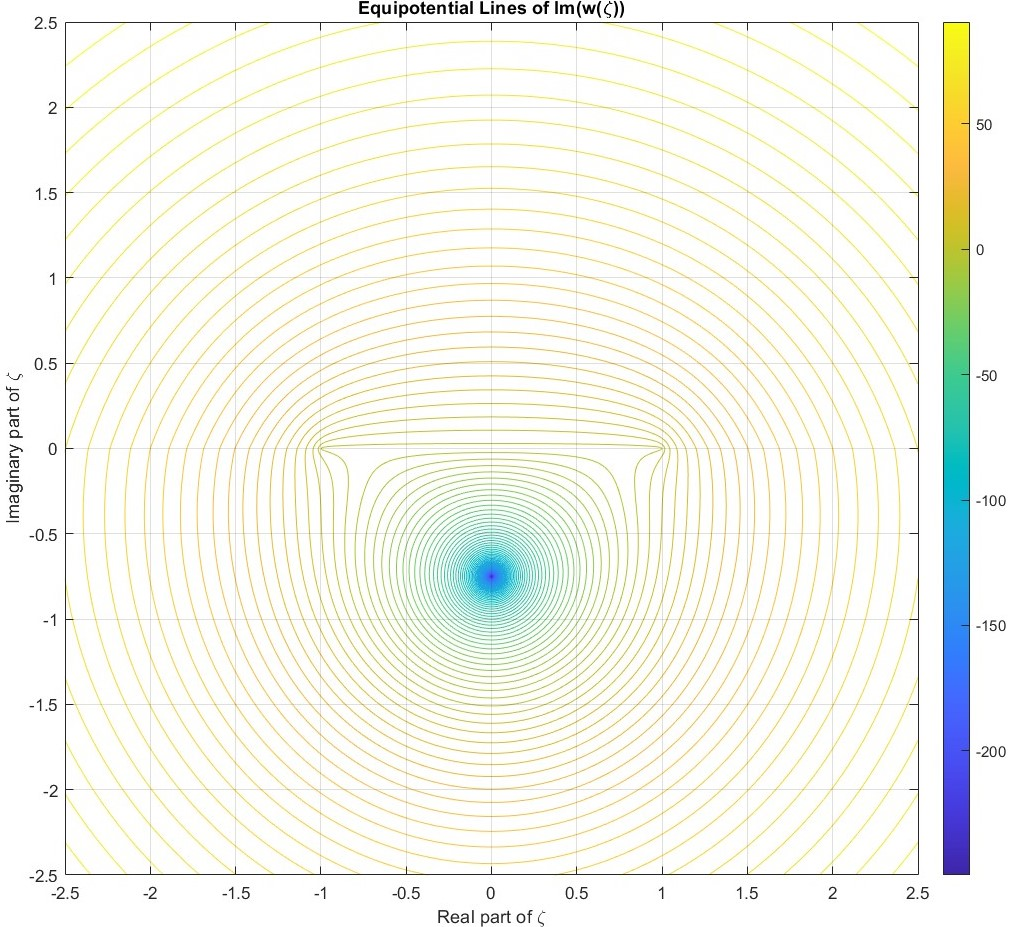
\includegraphics[width=1.\linewidth]{Figs/whole slit vot.jpg}
        \caption{\small The equipotentials of the entire plane are a combination of four parts. The slit is at $(\pm1,y=0)$. The induced charge is not seen. There is a slight distortion of voltages at $y=0$, the boundary between the dielectric and the region above.}
        \label{fig:enter-label}
    \end{figure}
 


\section{Summary}
    \hspace{0em}\indent This chapter discusses the boundary conditions for the electrodes, dielectric, and droplet problem, scaling it down to a thin film problem and further simplifying it to solve the Laplace and Poisson equations for the point charge and disc embedded in a dielectric. Subsequently, two models are established: one for the charged disc embedded in a dielectric and the another for a point charge embedded in a dielectric. 
    
    The shielding effect of the dielectric is derived, and conformal mapping methods are used to analyse the induced charge positions in a dielectric with specific symmetry. Based on these models and the conformal mapping technique, the complex potential for the charge, dielectric, and conductive slit is obtained, which also describes a distant conducting droplet in a point charge's electric field.
    
    In the process, complex analysis tools simplify the boundary conditions and the calculations of the electric field, aiding in the identification of induced charges. Whereas, when a dielectric is present, Gauss's Law at the dielectric boundary requires the use of electric field equations to determine the magnitude of the charge.

\pagebreak